\documentclass[12pt,a4paper]{report}

\usepackage[utf8]{inputenc}
\usepackage[english]{babel}
\usepackage{amsmath}
\usepackage{amsfonts}
\usepackage{amssymb}
\usepackage{graphicx}
\usepackage{cite}
\usepackage{hyperref}
\usepackage[left=2cm,right=2cm,top=2cm,bottom=2cm]{geometry}

\author{Boyan Naydenov}
\title{Communications Protocol}


\begin{document}
\maketitle

\chapter{Protocols}
\section{Introduction}
\subsection{Data Communications}
\paragraph{}

It is defined as the exchange of data between two devices via a transmission medium.\\

Its effectiveness is valued by the next requirements: Delivery, Accuracy, Timeliness (late data is not useful) and Jitter (variation in the packet arrival time).\newline

It is composed by the following parts:

\begin{itemize}
\item Message
\item Sender
\item Receiver
\item Transmission Medium
\item Protocol ( Set of rules that govern data communication. Represents an agreement between the communicating devices)
\end{itemize}

\textbf{Data Representation: }Different types of data as text, video, images or audio are represented by a group of bits, at their lowest level.
\newline

\textbf{Data Flow:} Can be simplex (one direction of communication), half-duplex (two directions but not simultaneous) and full duplex (both directions simultaneously).

\subsection{Networks}
\paragraph{} Set of devices (nodes) interconnected.\newline

It is designed with the next criteria: performance (more throughput, less delay), reliability and security.

\textbf{Physical Structures:}
\begin{itemize}
\item Type of connection: Can be Point-to-Point or multipoint.
\item 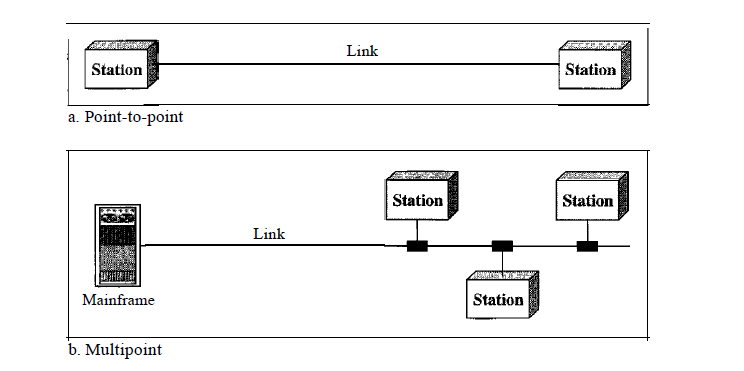
\includegraphics[scale=0.7]{p2p}
\item Physical Topology (refers to the way in which a network is laid out physically)
\begin{enumerate}

\item Mesh (point to point)
\begin{itemize}
\item\textit{Advantages:}A mesh offers several advantages over other network topologies. First, the use of dedicated links guarantees that each connection can carry its own data load, thus eliminating the traffic problems that can occur when links must be shared by multiple devices. Second, a mesh topology is robust. If one link becomes unusable, it does not incapacitate the entire system. Third, there is the advantage of privacy or security. When every message travels along a dedicated line, only the intended recipient sees it. Physical boundaries prevent other users from gaining access to messages. Finally, point-to-point links make fault identification and fault isolation easy. Traffic can be routed to avoid  links with suspected problems. This facility enables the network manager to discover the precise location of the fault and aids in finding its cause and solution.
\item\textit{Disadvantages:}complex and expensive.
\item 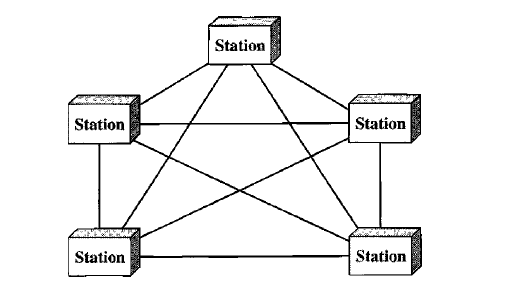
\includegraphics[scale=0.7]{mesh}
\end{itemize}

\item Star (point to point)
\begin{itemize}
\item\textit{Advantages:}cheaper than mesh (each device needs only one I/O), easy to install and reconfigure, robustness (if one link fails, no other link is affected).
\item\textit{Disadvantages:}If the hub fails, the system dies. Used in LAN networks (Local Area Network)
\item 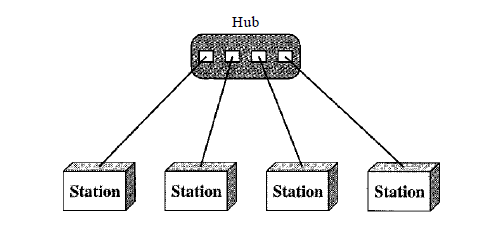
\includegraphics[scale=0.7]{star}
\end{itemize}

\item Bus (multipoint)
\begin{itemize}
\item\textit{Advantages:}
\item\textit{Disadvantages:}
\item 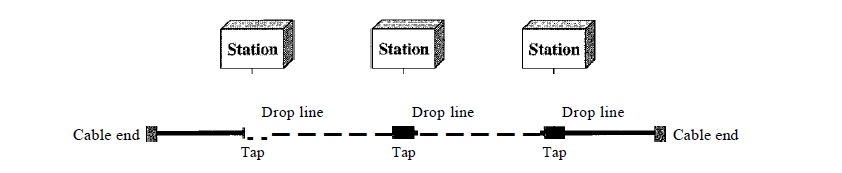
\includegraphics[scale=0.7]{bus}
\end{itemize}

\item Ring (multipoint)
\begin{itemize}
\item\textit{Advantages:}Easy to install and reconfigure, adding more devices is easy.
\item\textit{Disadvantages:}Unidirectional traffic, a break in the ring because of a disabled station can disable the entire network (can be solved by a double ring).
\item 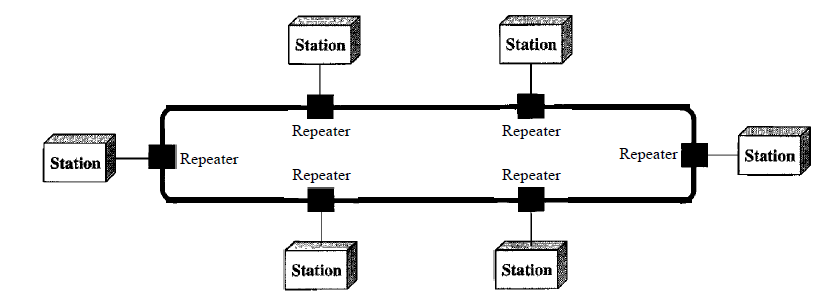
\includegraphics[scale=0.7]{ring}
\end{itemize}

\item Hybrid
\begin{itemize}
\item For example:
\item 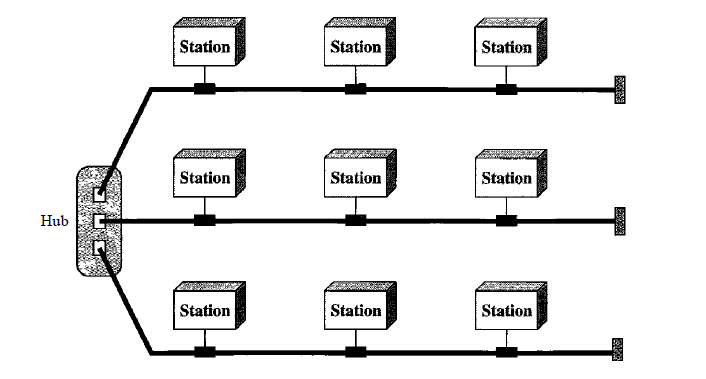
\includegraphics[scale=0.7]{hybrid}
\end{itemize}

\end{enumerate}
\end{itemize}
\textbf{Network Models:}
Standards are needed so that heterogeneous networks can communicate with one another. Best known standards are:
\begin{itemize}
\item Open Systems Interconnection (OSI) (7 layer network)
\item Internet Model (5 layer network)
\end{itemize}
\textbf{Categories of Networks: }
\begin{itemize}
\item LAN (local area network). Range limited to a few km.
\item WAN (wide area network). Long distance transmission of any data.
\item MAN (metropolitan area network). Intermediate size.
\end{itemize}
\textbf{Network Models:}
Standards are needed so that heterogeneous networks can communicate with one another. Best known standards are:
\begin{itemize}
\item Open Systems Interconnection (OSI) (7 layer network)
\item Internet Model (5 layer network)
\end{itemize}
\textbf{Interconnections of Networks: }Internetwork or Internet: Network of networks.


\subsection{Protocols}
Protocols and standards are what make networks work together. Protocols make it possible for the various components of a network to communicate with each other. Standards also make it possible for network components manufactured by different companies to work together.\newline

A protocol is a set of rules that enables effective communications to occur. One encounters protocols every day.\newline
\textbf{Key elements:}
\begin{itemize}
\item \textbf{Syntax}. Refers to the structure of the presented data. For example: first 8 bits show the sender address.
\item \textbf{Semantics}. Refers to the meaning of each section of bits.
\item \textbf{Timing}. Refers to: when data should be sent and how fast. If a sender produces 100Mbps and the receiver handles just 1Mbps, the receiver will be overloaded and data would be lost.
\end{itemize}
\textbf{Standards:}
\begin{itemize}
\item De facto (it has become a standard on its own )
\item De jure ( standards with official legislation backing them)
\end{itemize}

The standard creation committee for Space is called \href{https://public.ccsds.org/default.aspx}{\textbf{The Consultative Committee for Space Data Systems}}.  Their recommendations become later part of ISO. The books are open to the public on their website.
\section{Network Models}
It is composed by hardware and software. The software part is very important as doing everything only with hardware could be very tedious.
\subsection{Layered Tasks}
To understand the layered tasks concept the following common situation is presented: \newline
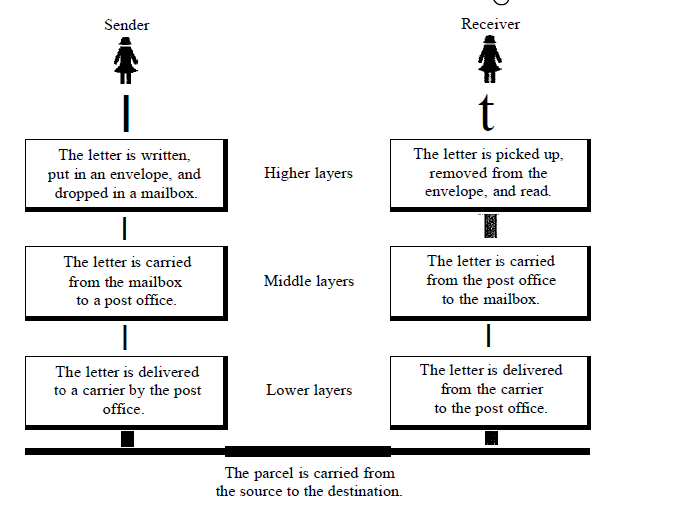
\includegraphics[scale=1]{layers} \newline
Note that a hierarchy is respected. For instance, the parcel cannot be carried before it has arrived to the post office, delivered by the sender. 
\subsection{The OSI Model}
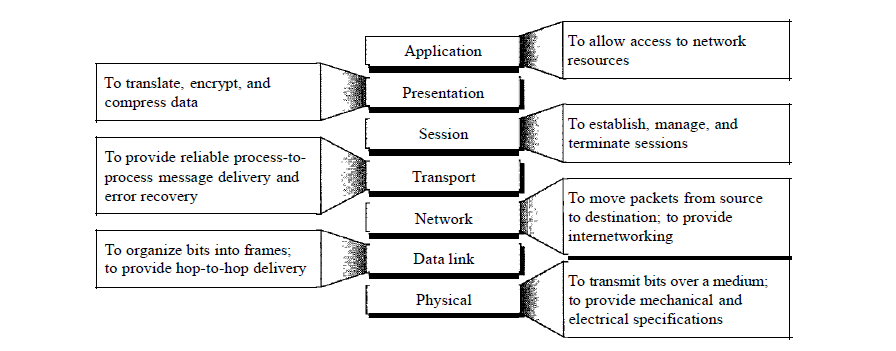
\includegraphics[scale=1]{osi} \newline
\subsection{TCP/IP Protocol Suite}
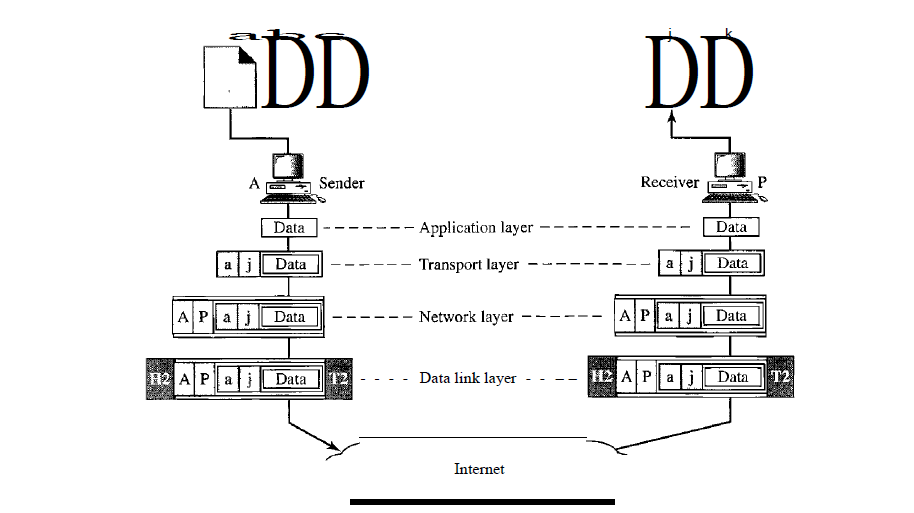
\includegraphics[scale=0.7]{ip_tcp} \newline
Some explanations:
\begin{itemize}
\item \textbf{Segments} are units of data in the Transport Layer (TCP/UDP in case of the Internet)
\item \textbf{Packets or Datagram}s are units of data in the Network Layer 
\item\textbf{ Frames} are units of data in the Link Layer (e.g. Wifi, Bluetooth, Ethernet, etc).

\end{itemize}
The Cubesat Space Protocol (CSP) is based in this model.
\section{Satellite Networks}
\paragraph{}A satellite network is a combination of nodes, some of which are satellites, that provides communication from one point on the Earth to another. A node in the network can be a satellite, an Earth station, or an end-user terminal or telephone.\newline

\textbf{Teledesic:}
Teledesic has 288 satellites in 12 LEO orbits, each at an altitude of 1350 km.
The system provides three types of communication. Intersatellite communication allows eight neighboring satellites to communicate with one another. Communication is also possible between a satellite and an Earth gateway station. Users can communicate directly with the network using terminals. Earth is divided into tens of thousands of cells. Each cell is assigned a time slot, and the satellite focuses its beam to the cell\newline

Transmission occurs in the \textbf{Ka bands (30Ghz)}.\newline

The data rate is up to \textbf{155 Mbps for the uplink and up to 1.2 Gbps for the downlink.}

\end{document}
